\chapter{The evolving matrix eigenvalue problem}		\label{Sec:evol_mats}



\section{Introduction}   \label{Subsec:evol_mats-intro}


In this chapter we examine the \textit{evolving matrix eigenvalue problem} (EMEP) in Algorithm \ref{Alg:PGD}.  
Section \ref{Subsec:evol_mats-spectral_props} defines the EMEP and examines its evolving spectrum across matrix iterates $A_k$.  
In particular, we observe that the algebraically largest eigenvalues tend to cluster as the algorithm proceeds, leading to more difficult eigenvalue problems for later matrix iterates.  
To handle these eigenvalue problems, we review the \textit{implicitly restarted Arnoldi method} (IRAM) \cite{sorensen1992implicit} in Section \ref{Subsec:evol_mats-IRAM}.  
The convergence behavior of the IRAM is based on the spectrum of the given eigenvalue problem as well as the IRAM parameters chosen by the user.
To understand and exploit the convergence behavior of the IRAM, we will review this method systematically from its component methods.









\section{The EMEP: computational costs and spectral properties}		\label{Subsec:evol_mats-spectral_props}


In this section we examine the sequence of eigenvalue problems in Algorithm \ref{Alg:PGD}, which we define as the \textit{evolving matrix eigenvalue problem} (EMEP).
We will see that the EMEP is the most computationally expensive subroutine in Algorithm \ref{Alg:PGD}.  
We also observe that the EMEP matrix iterates have a spectrum which evolves in a predictable way from early to later iterates.


We begin by formally defining the EMEP.
Generally speaking, we are concerned with a sequence of eigenvalue problems in which each eigenvalue problem is dependent on the results of the previous problems.  
For each iterate $k$ in this sequence of problems, we have some Hermitian matrix iterate $A_k \in \caH^n$ and seek its $j$ algebraically largest eigenvalues $\Lambda^{(k)}_j$ and the corresponding eigenvectors $V^{(k)}_j$.  
%Next, the previous set of basis matrices $\caV_{k} = \{ V^{(i)}_j \}_{i=0}^{k}$ are used to find the next matrix iterate $A_{k+1}$.  
%More specifically, we are concerned with problems of the form
%\begin{equation} 		\label{Eqn:EMEP_general}
%\begin{array}{ll}
%\textnormal{for}
%	&	k = 1, 2, \ldots, K		\\
%\textnormal{find}	
%	&	\left( \Lambda^{(k)}_j, \ V^{(k)}_j \right) \textnormal{ of } A_k
%\end{array}
%\end{equation}
%where $\Lambda^{(k)}$ are the $j$ algebraically largest eigenvalues of $A_k$, $V_k$ is the matrix of corresponding eigenvectors, $A_k \in \caH^n$ is dependent on $\caV_{k} = \{ V^{(i)}_j \}_{i=0}^{k}$, and $V_0 \in \bbC^{n \times j}$ is an initial basis matrix.
Some examples of this problem include subspace tracking in signal processing (see, e.g., \cite{comon1990tracking}, \cite{stewart1992updating}, \cite{yang1995projection}, \cite{doukopoulos2008fast}), matrix completion (e.g., \cite{ngo2012scaled}), and the Kohn-Sham equation in density functional theory (e.g., \cite{saad2010numerical}).

%Subspace tracking. Possibly the best known use of subspace iteration for evolving matrices is in the context of “subspace tracking” in signal processing applications; see, e.g., [6, 21, 2, 7]. An excellent survey of relatively recent work on the topic can be found in the introduction of [7]. The problem here is to track the “signal subspace,” which is the eigenspace associated with the largest eigenvalues of a covariance matrix associated with a sequence of signals, in the form of vectors x(t),t ∈ Z, that are being received sequentially. 
%Matrix completion. Another notable application where subspace iteration with evolving matrices plays a major role [14] is that of the matrix completion problem.
%For example, in the “nonlinear eigenvector problem” that is at the heart of density functional theory (DFT) (see, e.g., [20]), one seeks the lowest eigenmodes of a Hamiltonian that depends (nonlinearly) on its eigenvectors
%DFT studies the electronic structure of materials by solving a simplified version of the Schro ̈dinger equation known as the Kohn–Sham equation:


To see that each eigenvalue problem in Algorithm \ref{Alg:PGD} is dependent on the results of the previous eigenvalue problems, first note that each eigenvalue problem in Algorithm \ref{Alg:PGD} (steps 2, 6, and 14) requires the two algebraically largest eigenvalues of the matrix iterate $A_k = \caA^*y_k$.  (Also note that the iterate $k$ does not correspond to the iterate number in Algorithm \ref{Alg:PGD} because step 6 involves a linesearch which may involve more than one eigenvalue problem.)  
We will show that each matrix iterate $A_k = \caA^*y_k$ in Algorithm \ref{Alg:PGD} is computed using a variable $y_k$ which is dependent on the previous set of basis vectors $\caV_{k-1} = \{ v_1^{(i)} \}_{i=0}^{k-1}$.  It can be shown inductively that $y_k$ is a function of $\caV_{k-1}$.  The initial iterate $k = 0$ corresponds to the first eigenvalue problem in Algorithm \ref{Alg:PGD}, where $y_0 = \Pi_\caC(b)$ is initialized using the observation vector $b$ and is independent of any eigenvector.  Thus we initialize $v_1^{(0)}$ as the empty set.  If $k >0$ then the update $y_k$ is computed as $y_k = \Pi_{\caC}(y_{k-1}- \alpha_{k-1}  g_{k-1})$, where $g_{k-1} = \caA(v_{k-1} v_{k-1}^*)$ is a function of $v_{k-1}$ and $\alpha_{k-1}$ is determined using a linesearch on the minimization problem
\begin{equation}
\begin{array}{ll}
\min\limits_{\substack{\alpha}}
	&	\lambda_1 \left( \caA^* ( \Pi_\caC ( y_{k-1} - \alpha g_{k-1} ) )  \right).
\end{array}
\end{equation}
As a result, $y_k$ is dependent on $v_{k-1}$ and $y_{k-1}$; and thus each eigenvalue problem in Algorithm \ref{Alg:PGD} is dependent on the results of the previous eigenvalue problems.

Thus we define the sequence of eigenvalue problems generated by Algorithm \ref{Alg:PGD} as the \textit{evolving matrix eigenvalue problem} (EMEP)
\begin{equation}		\label{Eqn:EMEP_PLGD}
\begin{array}{ll}
\textnormal{for}
	&	k = 1, 2, \ldots, K		\\
\textnormal{find}	
	&	\left( \lambda^{(k)}_1, \ v^{(k)}_1 \right) \textnormal{ and } \left( \lambda^{(k)}_2, \ v^{(k)}_2 \right) \textnormal{ of } A_k,
\end{array}
\end{equation}
where $\lambda^{(k)}_1$ and $\lambda^{(k)}_2$ are the two algebraically largest eigenvalues of the \textit{matrix iterate} $A_k = \caA^*y_k$, and $y_k$ is the previous dual variable generated by Algorithm \ref{Alg:PGD} (from step 2, 6, or 14).



Next, we examine the overall computational costs of the \emep.
As discussed in Section \ref{Subsec:PLGD_algo-algo}, the main computational costs in Algorithm \ref{Alg:PGD} are the EMEP (step 2, 6, and 14), the primal refinement (step 11), and the dual refinement (step 13).  
Since we are focused on PLGD models with Gaussian noise (\ref{Eqn:PhaseLift-GD_Gaussian_noise}), the dual refinement step of Algorithm \ref{Alg:PGD} is skipped (see the end of Section \ref{Subsec:PLGD_term_crit-stagnation} for an explanation).
In both the \emep \ and the primal refinement step, the primary computational cost comes from $\caA$-products (\ref{Eqn:A_definition_with_masks}), where each $\caA(xx^*)$ product requires $L$ DFTs and each $[\caA^*y]x$ product requires $2L$ DFTs.  
Thus we measure computational costs in terms of the number of DFTs, following the convention of \cite{DBLP:journals/tit/CandesLS15} and \cite{DBLP:journals/siamsc/FriedlanderM16}.
Also note that the computation of the eigenpair $(\lambda_1, v_1)$ in the \emep \ must be very accurate in order to determine an accurate descent step $g = \caA(v_1v_1^*)$ in Algorithm \ref{Alg:PGD}.
Table \ref{Tab:EMEP_costs} depicts the number of DFTs in Algorithm \ref{Alg:PGD} for a variety of noisy problems.
\begin{table}[H]
\centering
\begin{footnotesize}
\hbox{

\hspace{-0.7cm}
\begin{tabular}{ |ccc|ccc|cc|cc| }
 \hline
			&&&  \multicolumn{3}{c|}{EMEP} 
			&  \multicolumn{2}{c|}{Primal refinement}
			& 	\multicolumn{2}{c|}{All other steps}	\\
$n$ & $L$ & $\epsilon_\text{rel}$ 	& \texttt{eigs} calls  & Minutes & DFTs & Minutes  & DFTs & Minutes  & DFTs   \\
 \hline
 4,096 &  5 & 0.05 & 228 & 13.13  (0.94) &  51,935  (0.97) & 0.73  (0.05) &   1,516  (0.03) & 0.04 &     17 	\\
 4,096 &  5 & 0.15 & 120 & 6.63  (0.94) &  31,085  (0.97) & 0.45  (0.06) &   1,076  (0.03) & 0.01 &     10 \\
 4,096 &  5 & 0.30 &  52 & 3.56  (0.89) &  16,410  (0.95) & 0.45  (0.11) &    854  (0.05) & 0.01 &      4 \\
 4,096 & 10 & 0.05 & 190 & 12.06  (0.96) &  72,587  (0.98) & 0.45  (0.04) &   1,819  (0.02) & 0.03 &     29	\\ 
 4,096 & 10 & 0.15 & 106 & 8.60  (0.96) &  51,450  (0.98) & 0.30  (0.03) &   1,194  (0.02) & 0.02 &     17 \\
 4,096 & 10 & 0.30 & 111 & 17.95  (0.98) & 107,936  (0.99) & 0.36  (0.02) &   1,420  (0.01) & 0.01 &     18 \\
 \hline
16,384 &  5 & 0.05 & 199 & 46.09  (0.95) &  69,745  (0.98) & 2.13  (0.04) &   1,468  (0.02) & 0.06 &     16	\\
16,384 &  5 & 0.15 &  91 & 27.71  (0.95) &  41,880  (0.98) & 1.34  (0.05) &    853  (0.02) & 0.03 &      8	\\
16,384 &  5 & 0.30 &  61 & 30.95  (0.94) &  45,834  (0.98) & 2.04  (0.06) &   1,026  (0.02) & 0.02 &      5	\\
16,384 & 10 & 0.05 & 160 & 56.73  (0.97) &  92,391  (0.98) & 1.64  (0.03) &   1,560  (0.02) & 0.07 &     25	\\
16,384 & 10 & 0.15 & 103 & 36.30  (0.97) &  60,189  (0.98) & 1.21  (0.03) &   1,167  (0.02) & 0.05 &     17	\\
16,384 & 10 & 0.30 &  47 & 18.48  (0.96) &  30,498  (0.98) & 0.65  (0.03) &    617  (0.02) & 0.02 &      8	\\
 \hline
\end{tabular}

}
\end{footnotesize}
\caption{Algorithm \ref{Alg:PGD} runtime and number of DFTs (with percentage of the total in parentheses) for the \emep, primal refinement (solving (\ref{Eqn:GD-PFD}) in step 11) and all other operations. Here $n$ is signal size (i.e., number of pixels squared in the image from Figure \ref{Fig:parrot_signal_iterates}), $L$ is number of observations, and $\epsilon_\textnormal{rel}$ is the noise ratio.} \label{Tab:EMEP_costs}
\end{table}
% experiments.figure.noisyimage_costs


The results in Table \ref{Tab:EMEP_costs} demonstrate the essential computational challenges of Algorithm \ref{Alg:PGD}.  First, the EMEP is the dominant computational cost in the algorithm, and its proportion to other costs (in both runtime and number of DFTs) increases as the size of the model increases.  Additionally, the primal refinement step requires a small but nontrivial amount of computation.  All other operations accounted for $0.00\%$ of the overall runtime. 



We will now profile the cost of the \emep.
Figure \ref{Fig:EMEP_costs_num_mat_vecs} depicts the number of matrix-vector products $[\caA^*y_k]x$ in the \emep \ for each of the six smaller models from Table \ref{Tab:EMEP_costs}. 

\begin{figure}[H]
\centering
\hbox{\hspace{-1.9cm} 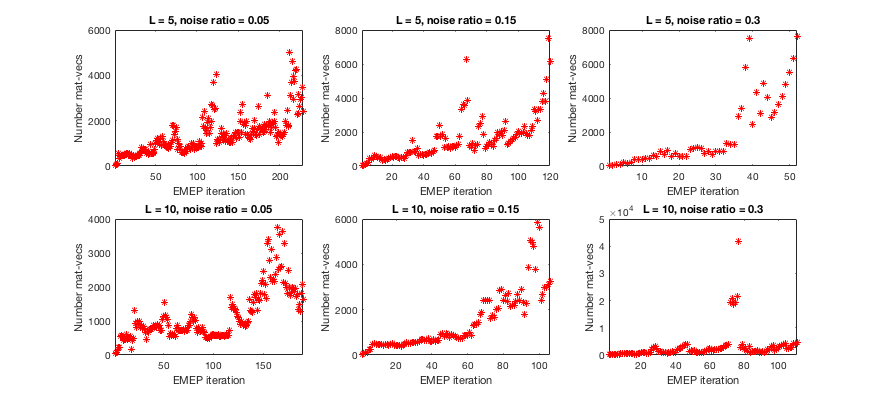
\includegraphics[scale=0.6]{EMEP_costs_num_mat_vecs} }\vspace{-0.4cm}
	\caption{Number of matrix-vector products for each iteration in the \emep \ for the six smaller models from Table \ref{Tab:EMEP_costs}	.}
\label{Fig:EMEP_costs_num_mat_vecs}
\end{figure}
% experiments.figure.noisyimage_costs

Figure \ref{Fig:EMEP_costs_num_mat_vecs} demonstrates that the number of matrix-vector products required for each \emep \ iterate varies greatly from earlier to later iterates.  In each model, the later iterates account for the majority of the computational cost of the \emep.  




To understand why the number of matrix-vector products increases as the \emep \ progresses, we close this section by examining the evolving spectrum distribution of these eigenvalue problems.  
Figure \ref{Fig:EMEP_full_spectrum} depicts the spectrum of earlier and later iterates for a particular model from Table \ref{Tab:EMEP_costs}.



\begin{figure}[H]
\centering
\hbox{\hspace{-1.9cm} 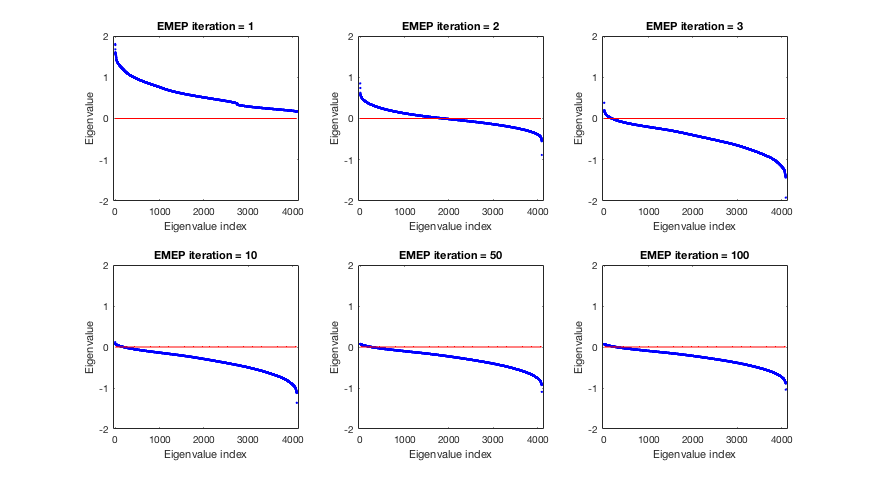
\includegraphics[scale=0.6]{EMEP_full_spectrum} }\vspace{-0.4cm}
	\caption{Spectrum of specific \emep \ matrix iterates $A_k$ for the model from Table \ref{Tab:EMEP_costs} with signal size $n = 4,096$, oversampling $L = 5$, and noise ratio $\epsilon_\text{rel} = 0.15$.}
\label{Fig:EMEP_full_spectrum}
\end{figure}
% experiments.figure.noisyimage_spectrumdist

As we see in Figure \ref{Fig:EMEP_full_spectrum}, the spectrum of the matrix iterates $A_k$ in the \emep \ shifts from completely positive for $A_1$ to mostly negative for later iterates.  This shift in spectrum is a consequence of optimizing the PLGD model (\ref{Eqn:PhaseLift-P-GD}).  The first matrix iterate $A_1 = \caA^*b$ will always be positive-semidefinite because the components of the observation $b=[b_1; b_2; \ldots; b_L]$ are all nonnegative and thus for all $x$ we have 
\[
x^*[\caA^*b]x 
	= \sum\limits_{\substack{j=1}}^{\substack{L}}
		[FC_jx]^* \textnormal{Diag}(b_j) F C_jx
	\geq 0.
\]
Since Algorithm \ref{Alg:PGD} minimizes the objective function $\lambda_1(\caA^*y_k)$, the algebraically largest eigenvalue $\lambda_1^{(k)}$ of $\caA^*y_k$ can be expected to decrease for later iterates $k$.  


As we will see in Section \ref{Subsec:evol_mats-IRAM}, the convergence rate of eigenvalue methods often depends on the distance between the desired eigenvalue $\lambda_j$ and the next algebraically largest eigenvalue $\lambda_{j+1}$.  Figure \ref{Fig:EMEP_largest_eigvals} depicts the 20 algebraically largest eigenvalues of the \emep \ iterates from Figure \ref{Fig:EMEP_full_spectrum}.


\begin{figure}[H]
\centering
\hbox{\hspace{-1.9cm} 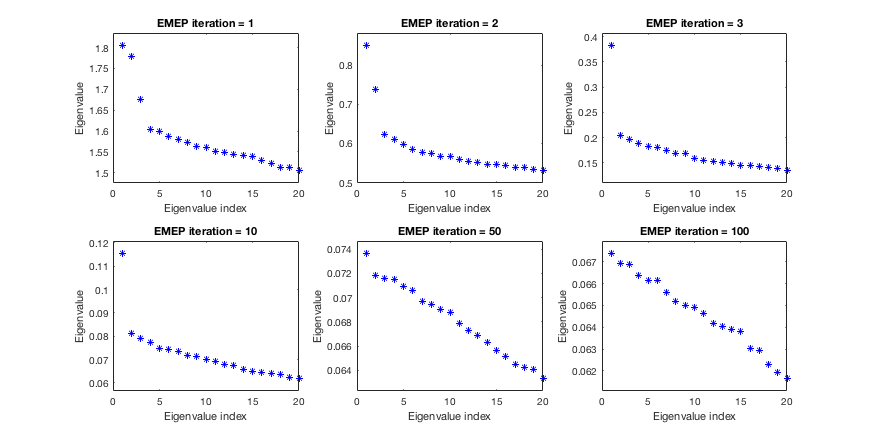
\includegraphics[scale=0.6]{EMEP_largest_eigvals} }\vspace{-0.4cm}
	\caption{Twenty algebraically largest eigenvalues of specific \emep \ matrix iterates $A_k$ for the model from Table \ref{Tab:EMEP_costs} with signal size $n = 4,096$, oversampling $L = 5$, and noise ratio $\epsilon_\text{rel} = 0.15$.}
\label{Fig:EMEP_largest_eigvals}
\end{figure}
% experiments.figure.noisyimage_spectrumdist

Figure \ref{Fig:EMEP_largest_eigvals} demonstrates that the algebraically largest eigenvalues of the matrix iterates $A_k$ cluster together as the \emep \ progresses.  
In general, this clustering in the \emep \ spectrum is expected.  
Section \ref{Subsec:PLGD_term_crit-stagnation} demonstrated that PLGD models with Gaussian noise (\ref{Eqn:PhaseLift-GD_Gaussian_noise}) typically have optimal primal matrices $X_\star$ with rank greater than one (see Table \ref{Tab:average_rank_soln_matrix_with_gaussian_dual_variable}).
And Corollary \ref{Cor:PLGD-optimality} (e) indicates that $\text{rank}(X_\star)$ is a lower bound on the multiplicity $r$ of the algebraically largest eigenvalue of the optimal dual matrix $\caA^*y_\star$.
Thus for later \emep \ iterates $k$, we can expect some $r$ algebraically largest eigenvalues $\lambda_1^{(k)}, \lambda_2^{(k)}, \ldots, \lambda_r^{(k)}$ to have a decreasing relative difference
\[
\frac{\lambda_i^{(k)} - \lambda_{i+1}^{(k)}}
	{\lambda_i^{(k)}}
\]
for $i = 1, 2, \ldots, r-1$.



The clustering of the algebraically largest eigenvalues as depicted in Figure \ref{Fig:EMEP_largest_eigvals} is known to slow the convergence rate of eigenvalue methods like the IRAM.
Yet the choice of the parameters in the IRAM can also have a significant effect on the convergence rate of the IRAM.
A thorough understanding of the IRAM and its subroutines will help us to develop a new, adaptive strategy for choosing IRAM parameters for the \emep \ in Chapter \ref{Sec:Numerics}.
Thus we proceed to review the IRAM.






\section{The implicitly restarted Arnoldi method}		\label{Subsec:evol_mats-IRAM}



% See following as references:
% http://www.cs.cornell.edu/~bindel/class/cs6210-f09/lec34.pdf
% http://people.inf.ethz.ch/arbenz/ewp/Lnotes/chapter11.pdf
%		Summarizes algorithms, math, convergence criteria, etc.
% ARPACK USERS GUIDE, p 53
%		Algo for IRAM on p 63

% Note: 
%	Prev	Golub
%	p		k, m
%	k		j
%	m		p (= m - j)
%	v		q


In this section we review the \textit{implicitly restarted Arnoldi method} (IRAM), a common large-scale eigenvalue method.  
First proposed by Sorensen \cite{sorensen1992implicit}, \cite{sorensen1997implicitly}, the IRAM is a combination of two essential algorithms.  
The \textit{$m$-step Arnoldi iteration} is used to build a matrix $Q_m$ of $m$ basis vectors which approximates the desired eigenspace.  
The \textit{$p$-step shifted QR iteration} restarts the matrix $Q_m$ with a specific strategy to damp unwanted eigenvalues, resulting in a smaller matrix $Q_j$ of $j<m$ basis vectors.  
Since the $m$-step Arnoldi iteration is an extension of the \textit{power method}, we first discuss the Power method before developing the IRAM.  
Altogether, the algorithms in this section are presented in the order depicted in Figure \ref{Fig:IRAM_flowchart}.

\begin{figure}[H] 
\centering
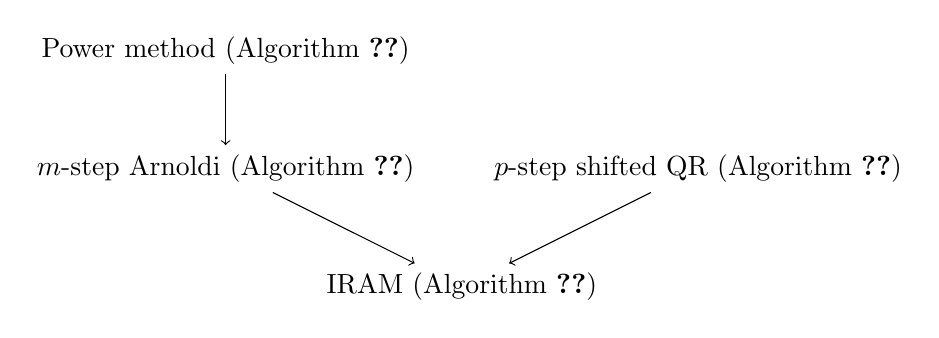
\begin{tikzpicture}
	\node (1) at (0,3) {Power method (Algorithm \ref{Alg:power_method})};
	\node (2) at (0,1.5) {$m$-step Arnoldi (Algorithm \ref{Alg:Arnoldi_iteration})};
	\node (3) at (6,1.5) {$p$-step shifted QR (Algorithm \ref{Alg:shifted_QR_iteration})};
	\node (4) at (3,0) {IRAM (Algorithm \ref{Alg:IRAM})};
	\draw[->] (1) -- (2);
	\draw[->] (2) -- (4);
	\draw[->] (3) -- (4);
\end{tikzpicture}
\caption{Dependency chart for the IRAM.}
\label{Fig:IRAM_flowchart}
\end{figure}

This section follows the treatment found in \cite[Chapters 8, 10]{golub2012matrix}, with occasional minor changes in notation.






The first method we consider is the \textit{power method}, a method for determining the largest magnitude eigenvalue $\lambda_1$ and corresponding eigenvector $v_1$ of a Hermitian matrix $A$.  The power method is based on the property that if $\lambda_1$ is strictly larger in magnitude than the next largest magnitude eigenvalue and the initial vector $q^{(0)}$ has a nonzero component in the direction of $v_1$ (i.e., $v_1^*q^{(0)} \neq 0$), then the sequence
\[
q^{(0)}, \frac{Aq^{(0)}}{||Aq^{(0)}||},  \frac{A^2q^{(0)}}{||A^2q^{(0)}||},  \frac{A^3q^{(0)}}{||A^3q^{(0)}||}, \ldots
\]
will have $v_1$ as its limit.  

Formally, Algorithm \ref{Alg:power_method} presents the power method as seen in \cite[Section 8.2.1]{golub2012matrix}.

\begin{algorithm}[H]
\caption{Power method}	\label{Alg:power_method}

\begin{algorithmic}[1]
	\Statex 	\textbf{Input:} Hermitian matrix $A$, initial approximate eigenvector $q^{(0)}$, relative tolerance $\textnormal{tol}_\textnormal{rel} > 0$.
	\Statex 	\textbf{Output:} Approximate largest magnitude eigenvalue $\lambda$ and the corresponding eigenvector $v$.
	\State		\textit{Initialize:} $q^{(0)} = q^{(0)}/||q^{(0)}||$, $\rho^{(0)} = [q^{(0)}]^*Aq^{(0)}$, $r^{(0)} = Au^{(0)} - \rho^{(0)}q^{(0)}$, $i= 1$.
	\While {\textit{not converged:} $ ||r^{(i)} || / (||Aq^{(i)}|| + |\rho^{(i)}|) > \textnormal{tol}_\textnormal{rel} $}
		\State		$z^{(i)} = Aq^{(i-1)}$
		\State		$q^{(i)} = z^{(i)} / ||z^{(i)}||$
		\State		$\rho^{(i)} = [q^{(i)}]^* z^{(i)}$
		\State		$r^{(i)} = Aq^{(i)} - \rho^{(i)}q^{(i)}$, $i = i + 1$
	\EndWhile
	\State		\textit{Return:} $(\lambda, v) = (\rho^{(i-1)} , q^{(i-1)})$.
\end{algorithmic}

\end{algorithm}


The simplicity of power method allows for insightful convergence results like the Theorem \ref{Thm:power_method_conv_rate}, in which we assume the matrix $A$ is real for clarity.

\begin{theorem}			\label{Thm:power_method_conv_rate}
Suppose $A \in \bbR^{n \times n}$ is symmetric with an eigenvalue decomposition
\[
V^*AV = \text{Diag}(\lambda_1, \lambda_2, \ldots, \lambda_n),
\]
where $V = [\ v_1 \ | \ v_2 \ | \cdots | \ v_n \ ]$ is orthogonal and $|\lambda_1| > |\lambda_2| \geq \cdots \geq |\lambda_n|$.  Let the vectors $q^{(i)}$ be generated by Algorithm \ref{Alg:power_method} and define $\theta_i \in [0, \pi/2]$ as 
\[
	\cos(\theta_i) = \left| v_1^Tq^{(i)} \right|.
\]
If $\cos(\theta_0) \neq 0$, then for $i = 0, 1, \ldots$ we have 
\begin{equation} 		\label{Eqn:power_method_conv_rate_1}
\left| \sin(\theta_i) \right| \leq \tan(\theta_0) \left| \frac{\lambda_2}{\lambda_1} \right|^i,
\end{equation}
\begin{equation} 		\label{Eqn:power_method_conv_rate_2}
\left| \lambda^{(i)} - \lambda_1 \right| \leq \max_{2 \leq j \leq n} \left| \lambda_1 - \lambda_i \right| \tan(\theta_0)^2 \left| \frac{\lambda_2}{\lambda_1} \right|^{2i}.
\end{equation}
\end{theorem}

\begin{proof}
See \cite[Theorem 8.2.1]{golub2012matrix}.
\end{proof}

Theorem \ref{Thm:power_method_conv_rate} establishes that the convergence rate of the power method (Algorithm \ref{Alg:power_method}) is dependent on the distance between $|\lambda_1|$ and $|\lambda_2|$.  If this distance $\epsilon = |\lambda_1| - |\lambda_2|$ is very small relative to $|\lambda_1|$, then we have
\[
\left| \frac{\lambda_2}{\lambda_1} \right| = \frac{|\lambda_1| - \epsilon}{|\lambda_1|} = 1 - \frac{\epsilon}{|\lambda_1|} \approx 1,
\]
and $|\sin(\theta_i)|$ in (\ref{Eqn:power_method_conv_rate_1}) may decreases very slowly.  








The next method we consider is the \textit{$m$-step Arnoldi iteration} which extends the power method (Algorithm \ref{Alg:power_method}) to achieve a superior convergence rate.  An iteration of the power method generates a new approximate eigenvector ($q^{(i)}$ from steps 3 and 4) by normalizing the matrix-vector product of the previous vector.  In essence, the power method searches for the largest magnitude eigenvalue $\lambda_1$ and corresponding eigenvector $v_1$ of a matrix $A$ in the one-dimensional subspace $V = \textnormal{span} \{ Aq_1 \}$.  The $m$-step Arnoldi iteration extends the power method by searching for the Ritz pair (\ref{Def:Ritz_pair_val_vec}) ($\theta_1, u_1$) for $A$ with respect to the $m$-dimensional \textit{Krylov subspace}
\begin{equation}
\caK_m(A, q_1) = \textnormal{span}\{ q_1, Aq_1, A^2q_1, \ldots, A^{m-1}q_1 \}.
\label{Def:krylov_subspace}
\end{equation}
Algorithm \ref{Alg:Arnoldi_iteration} (as described in \cite[Algorithm 10.5.1]{golub2012matrix}) builds a unitary basis $Q_m$ of $\caK_m(A, q_1)$ which may be used to find the Ritz pair ($\theta_1, u_1$).
\begin{algorithm}[H]
\caption{$m$-step Arnoldi iteration}	\label{Alg:Arnoldi_iteration}

\begin{algorithmic}[1]
	\Statex		\textbf{Input:} Matrix $A \in \bbC^{n \times n}$, number of Arnoldi steps $m$, initial approximate eigenvector $q_1$.
	\Statex 	\textbf{Output:} Hessenberg matrix $H_m$, basis $Q_m$, residual $r_m$.
	\State		\textit{Initialize:} $q_1  = q_1 / ||q_1||$, \ \ $z = Aq_1$, \ \ $\alpha_1 = q_1^*z$, \ \ $r_1 = z - \alpha_1 q_1$, \ \ $Q_1 = [q_1]$, \ \ $H_1 = [\alpha_1]$.
	\For 			{$i = 1, \ldots, m-1$}
		\State	$\beta_i = ||r_i||$, \ \ $q_{i+1} = r_i / \beta_i$.
		\State	$Q_{i+1} = [Q_i \ | \ q_{i+1}]$, \ \ $\hat{H}_i = \begin{bmatrix}	H_i \\  \beta_i e_i^T	\end{bmatrix}$.
		\State	$z = Aq_{i+1}$.
		\State	$h = Q_{i+1}^*z$, \ \  $r_{i+1} = z - Q_{i+1}h$.
		\State	$H_{i+1} = [\hat{H}_i \ | \ h]$.
	\EndFor
	\State		\textit{Return:} $H_m, Q_m, r_m$.
\end{algorithmic}

\end{algorithm}

In order to obtain a Ritz pair ($\theta, u$) for $A$ with respect to $\caK_m(A, q_1)$, the $m$-step Arnoldi iteration generates an \textit{$m$-step Arnoldi decomposition}
\begin{equation} 		\label{Eqn:Arnoldi_decomp}
AQ_m = Q_m H_m + r_m e_m^*,
\end{equation}
where $H_m$ is an upper Hessenberg matrix.  If $(\theta, w)$ is an eigenpair for $H_m$ and $u = Q_mw$ then (\ref{Eqn:Arnoldi_decomp}) implies
\begin{equation} 			\label{Eqn:Arnoldi_decomp_Ritz_pairs}
(AQ_m - Q_mH_m)w = (A-\theta I) u = (e_m^*w)r_m.
\end{equation}
Additionally, steps 5 and 6 of Algorithm \ref{Alg:Arnoldi_iteration} indicate that $r_m$ is orthogonal to $\caK_m(A, q_1)$, and thus ($\theta, u$) is a Ritz pair for $A$ with respect to $\caK_m(A, q_1)$.  


The use of $\caK_m(A, q_1)$ in Algorithm \ref{Alg:Arnoldi_iteration} allows for superior convergence to Algorithm \ref{Alg:power_method}.  Note that the largest magnitude Ritz pair $(\theta_1, u_1)$ for $A$ with respect to $\caK_m(A, q_1)$ generated by Algorithm \ref{Alg:Arnoldi_iteration}  is guaranteed to be at least comparable to the $m$-th iterate of Algorithm \ref{Alg:power_method} since $A^{m-1}q_1 \in  \caK_m(A, q_1)$.  To compare the convergence rates of Algorithms \ref{Alg:power_method} and \ref{Alg:Arnoldi_iteration} more precisely, assume the matrix $A$ in real and symmetric.  Then the matrix $H_m$ returned by Algorithm \ref{Alg:Arnoldi_iteration} is tridiagonal and this algorithm is equivalent to the \textit{$m$-step Lanczos iteration} \cite[Algorithm 10.1.1]{golub2012matrix}.  In this case, we have the Theorem \ref{Thm:Lanczos_conv_rate}.  Note that this theorem involves \textit{Chebyshev polynomials} \cite[Section 4.4]{saad2011numerical}, a sequence of polynomials defined recursively as
\begin{equation} 			\label{Def:Chebyshev_polys}
c_k(x) = 2x c_{k-1}(x) - c_{k-2}(x)
\end{equation}
for $k \geq 2$, with $c_0 = 1$ and $c_2 = x$ .

\begin{theorem}   		\label{Thm:Lanczos_conv_rate}
Let $A \in \bbR^{n \times n}$ be symmetric with an eigenvalue decomposition
\[
V^*AV = \text{Diag}(\lambda_1, \lambda_2, \ldots, \lambda_n),
\]
where $V = [\ v_1 \ | \ v_2 \ | \cdots | \ v_n \ ]$ is orthogonal and $\lambda_1 \geq \lambda_2 \geq \cdots \geq \lambda_n$.  Suppose the $m$-step Arnoldi iteration (Algorithm \ref{Alg:Arnoldi_iteration}) is performed and $H_k$ is the tridiagonal matrix returned by this algorithm.  If $\theta_1$ is the algebraically largest eigenvalue of $H_m$, then
\begin{equation} 			\label{Eqn:Lanczos_thm_1}
\lambda_1 \geq \theta_1 \geq \lambda_1 - (\lambda_1 - \lambda_n) 
\left( \frac{\tan(\phi_1)}{c_{m-1}(1+2\rho_1)} \right)^2,
\end{equation}
where $\cos(\phi_1) = |q_1^Tv_1|$,
\begin{equation}		\label{Eqn:Lanczos_thm_2}
\rho_1 = \frac{\lambda_1 - \lambda_2}{\lambda_2 - \lambda_n},
\end{equation}
and $c_{m-1}(x)$ is the Chebyshev polynomial of degree $m-1$.
\end{theorem}

\begin{proof}
See \cite[Theorem 10.1.2]{golub2012matrix}.
\end{proof}

The convergence rate established in Theorem \ref{Thm:Lanczos_conv_rate} may also be applied to Algorithm \ref{Alg:power_method}, giving the Corollary \ref{Cor:Lanczos_cor_for_power_method}.

\begin{corollary} 			\label{Cor:Lanczos_cor_for_power_method}
Let $A \in \bbR^{n \times n}$ be symmetric and positive semidefinite with an eigenvalue decomposition
\[
V^*AV = \text{Diag}(\lambda_1, \lambda_2, \ldots, \lambda_n),
\]
where $V = [\ v_1 \ | \ v_2 \ | \cdots | \ v_n \ ]$ is orthogonal and $\lambda_1 \geq \lambda_2 \geq \cdots \geq \lambda_n \geq 0$.  Suppose $m$ steps of the power method (Algorithm \ref{Alg:power_method}) are performed and $\gamma_1 = \rho^{(m)}$ is the returned Ritz value.  Then
\begin{equation} 			\label{Eqn:Lanczos_cor_for_power_method}
\lambda_1 \geq \gamma_1 \geq \lambda_1 - (\lambda_1 - \lambda_n) 
\tan^2(\phi_1) \left( \frac{\lambda_2}{\lambda_1} \right)^{2(m-1)},
\end{equation}
where $\cos(\phi_1) = |q_1^Tv_1|$.
\end{corollary}

\begin{proof}
See \cite[Theorem 10.1.2]{golub2012matrix} and replace the Chebyshev polynomial in this proof with $p(x) = x^{k-1}$.
\end{proof}


The lower bounds in Theorem \ref{Thm:Lanczos_conv_rate} and Corollary \ref{Cor:Lanczos_cor_for_power_method} may be used to compare the expected convergence rates for Algorithms \ref{Alg:power_method} and \ref{Alg:Arnoldi_iteration}.  The following comparison is based on \cite[Section 10.1.6]{golub2012matrix}.  Assume $A \in \bbR^{n \times n}$ is symmetric and also positive semidefinite for clarity.  Assume Algorithms \ref{Alg:power_method} and \ref{Alg:Arnoldi_iteration} have been run for $m$ steps with the same initial vector $q_1$.  Let $\gamma_1 = \rho^{(m)}$ be the Ritz value for $A$ generated by step 5 of Algorithm \ref{Alg:power_method}.  And let $\theta_1$ be the Ritz value for $A$ with respect to $\caK_m(A, q_1)$ generated by the algebraically largest eigenvalue of $H_m$ from Algorithm \ref{Alg:Arnoldi_iteration}.  Then we may compare the lower bounds (\ref{Eqn:Lanczos_cor_for_power_method}) for $\gamma_1$ and (\ref{Eqn:Lanczos_thm_1}) for $\theta_1$ by comparing the values
\begin{equation} 		\label{Eqn:power_method_lower_bound}
P_{m-1} = \left( \frac{\lambda_2}{\lambda_1} \right)^{2(m-1)},
\end{equation}
\begin{equation}  	\label{Eqn:Lanczos_lower_bound}
L_{m-1} 
	= \frac{1}{\left[c_{m-1}\left(2\frac{\lambda_1}{\lambda_2} -1 \right)\right]^2} 
	\geq 	\frac{1}{\left[ c_{m-1}\left( 1 + 2 \rho_1 \right) \right]^2}.
\end{equation}
Table \ref{Tab:Lanczos_vs_power_method} compares $P_{m-1}$ and $L_{m-1}$ for a few values of $m$ and $\lambda_1/\lambda_2$.

\begin{table}[H]
\centering
\begin{tabular}{ |c|cc|cc| }
 \hline

 	&	\multicolumn{2}{c|}{$m = 10$}
 		&	\multicolumn{2}{c|}{$m = 20$}	\\
 $\lambda_1 / \lambda_2$	&	$P_{m-1}$	&	$L_{m-1}$
 		&	$P_{m-1}$	&	$L_{m-1}$		\\ 			
 \hline
$1.10$
	&	$1.8 \times 10^{-1}$ & $5.5 \times 10^{-5}$
		&	$2.7 \times 10^{-2}$ & $2.1 \times 10^{-10}$	\\
$1.01$
	&	$8.4 \times 10^{-1}$ & $1.0 \times 10^{-1}$
		&	$6.9 \times 10^{-1}$ & $2.0 \times 10^{-3}$	\\
 \hline
\end{tabular}
\caption{Lower bound terms (\ref{Eqn:power_method_lower_bound}) and (\ref{Eqn:Lanczos_lower_bound}) for Ritz values generated by Algorithms \ref{Alg:power_method} and \ref{Alg:Arnoldi_iteration} } \label{Tab:Lanczos_vs_power_method}
\end{table}

Table \ref{Tab:Lanczos_vs_power_method} demonstrates that the use of the Krylov subspace $\caK_m(A, 	q_1)$ in Algorithm \ref{Alg:Arnoldi_iteration} allows for superior convergence to Algorithm \ref{Alg:power_method}.  Yet this superior convergence rate is slowed somewhat when the desired eigenvalue $\lambda_1$ is close to $\lambda_2$.  For eigenvalue problems where the value $\lambda_1 / \lambda_2$ is very small (like later iterates of the \emep, as demonstrated in Figure \ref{Fig:EMEP_largest_eigvals}), we may seek to increase the number of steps $m$ in Algorithm \ref{Alg:Arnoldi_iteration}.  Yet increasing $m$ can be computationally prohibitive if the eigenvalue problem is very large, requiring significant memory to store $Q_m$ and significant computation to compute the eigenvalue decomposition of $H_m$.






To take advantage of the convergence rate of Algorithm \ref{Alg:Arnoldi_iteration} for larger eigenvalue problems, the Arnoldi decomposition (\ref{Eqn:Arnoldi_decomp}) may be restarted with the \textit{$p$-step shifted QR iteration} developed by \cite{sorensen1992implicit} and discussed in \cite[Sections 10.5.2-3]{golub2012matrix}.  To develop this algorithm, assume we are seeking the $j$ algebraically largest eigenvalues of a Hermitian matrix $A \in \bbC^{n \times n}$ and we require that the $m$-step Arnoldi decomposition (\ref{Eqn:Arnoldi_decomp}) $AQ_m = Q_m H_m + r_m e_m^*$ has a fixed size $m > j$.  First we run Algorithm \ref{Alg:Arnoldi_iteration} with the initial vector $q_1$ to obtain $AQ_m = Q_m H_m + r_m e_m^*$.  Next, recall that the matrix $H_m$ may be used to identify the desired Ritz pairs $\{(\theta_i, u_i)\}_{i=1}^j$ for $A$ with respect to $\caK_m(A, q_1)$, as described in (\ref{Eqn:Arnoldi_decomp_Ritz_pairs}).  Yet $H_m$ also contains Ritz values $\theta_{j+1}, \ldots, \theta_m$ which correspond to unwanted eigenvalues of $A$.  To damp these unwanted Ritz values, we may select an appropriate degree $p = m-j$ filter polynomial $p(\lambda)$.  The $p$-step shifted QR iteration uses the filter polynomial
\begin{equation} 			\label{Eqn:filter_poly}
p(\lambda) = c \cdot (\lambda - \mu_1) (\lambda - \mu_2) \cdots (\lambda - \mu_p),
\end{equation}
where $c$ is a constant and the shift values $\mu_1 = \theta_{j+1}, \ldots, \mu_p = \theta_m$ are the $p$ unwanted Ritz values of $A$ with respect to $\caK_m(A, q_1)$.  Algorithm \ref{Alg:shifted_QR_iteration} (as described in \cite[Section 10.5.3]{golub2012matrix}) uses the filter polynomial (\ref{Eqn:filter_poly}) implicitly by applying $p$ shifted QR steps to $H_m$.
%(see \cite[Section 5.2]{golub2012matrix} for details regarding the QR factorization)
\begin{algorithm}[H]
\caption{$p$-step shifted QR iteration (implicit polynomial filtering)}	\label{Alg:shifted_QR_iteration}

\begin{algorithmic}[1]
	\Statex 	\textbf{Input:} Hessenberg matrix $H_m \in \bbC^{m \times m}$ and shift values $\mu_1, \ldots, \mu_p$.
	\Statex 	\textbf{Output:} Processed Hessenberg matrix $H_m^+ \in \bbC^{m \times m}$ and change of basis $V \in \bbC^{m \times m}$, with $H_m^+ = V^*H_mV$.
	\State		Set $H^{(0)} = H_m$.
	\For {$i = 1, \ldots, p$ }
		\State		\textit{QR factorization:} $H^{(i-1)} - \mu_i I = V_iR_i$.
		\State		\textit{Update:} $H^{(i)} = R_iV_i + \mu_iI$.
	\EndFor
	\State		Set $H_m^+ = H^{(p)}$, $V = V_1  V_2 \cdots V_p$.
	\State		\textit{Return:} $H_m^+, V$.
\end{algorithmic}

\end{algorithm}

Proposition \ref{Prop:Arnoldi_restart} establishes that Algorithm \ref{Alg:shifted_QR_iteration} implicitly applies the filter polynomial $p(\lambda)$ from (\ref{Eqn:filter_poly}) to the initial vector $q_1$ used to create the $m$-step Arnoldi decomposition (\ref{Eqn:Arnoldi_decomp}).

\begin{prop} 			\label{Prop:Arnoldi_restart}
Let $A \in \bbC^{n \times n}$ be Hermitian and $AQ_m = Q_mH_m + r_me_m^*$ be the $m$-step Arnoldi decomposition (\ref{Eqn:Arnoldi_decomp}) returned by Algorithm \ref{Alg:Arnoldi_iteration} with initial vector $q_1$.  And let $\mu_1, \ldots, \mu_p$ be the $p$ smallest algebraic eigenvalues of $H_m$.  Run Algorithm \ref{Alg:shifted_QR_iteration} with $H_m$ and $\mu_1, \ldots, \mu_p$ as inputs, and return $H_m^+$, $V = V_1 \cdots V_p$, and $R = R_p \cdots R_1$.

Then the restarted matrix $Q_+ = Q_mV$ will have the first column
\[
q_+ = Q_mV(:,1) = p(A)q_1,
\]
where $p(\lambda)$ is the filter polynomial (\ref{Eqn:filter_poly}) with constant $c = 1/R(1,1)$.
\end{prop}


\begin{proof}
See \cite[Section 10.5.3]{golub2012matrix}.
\end{proof}


\iffalse

\begin{proof}
First we must show that 
\begin{equation} 		\label{Eqn:filter_poly_proposition-VR}
VR = (H_m - \mu_1I) \cdots (H_m - \mu_pI).
\end{equation}

Using induction, we see that if $p=1$ then clearly (\ref{Eqn:filter_poly_proposition-VR}) holds.  If $p>1$, then let $\tilde{V}=V_1 \cdots V_{p-1}$ and $\tilde{R} = R_{p-1} \cdots R_1$, and note that $H^{(p-1)} = \tilde{V}^*H_m\tilde{V}$.  Then we have
\[
\begin{split}
VR & = \tilde{V}(V_pR_p)\tilde{R} 
	= \tilde{V} \left( H^{(p-1)} - \mu_pI \right) \tilde{R}
	= \tilde{V}\left( \tilde{V}^*H_m \tilde{V} - \mu_p I \right)\tilde{R}	\\
	& = \left(H_m - \mu_p I \right) \tilde{V}\tilde{R}
	= (H_m - \mu_p I) (H_m - \mu_1 I) \cdots (H_m - \mu_{p-1}I) 	\\
	&=  (H_m - \mu_1I) \cdots (H_m - \mu_pI),
\end{split}
\]
and (\ref{Eqn:filter_poly_proposition-VR}) holds.

Next, note that if the $m$-step Arnoldi decomposition (\ref{Eqn:Arnoldi_decomp}) is right-multiplied by $e_1$, then for all $\mu$ we have
\begin{equation} 			\label{Eqn:filter_poly_propostion-flip}
\left(A - \mu I \right)Q_me_1 = Q_m \left(H_m - \mu I \right) e_1.
\end{equation}

Then we have
\[
\begin{split}
q_+ 
	& = Q_mV(:,1) = Q_m \left[ \frac{1}{R(1,1)}VR e_1 \right] 	\\
	& 	= Q_m p(H_m) e_1 = p(A)Q_m e_1	\\
	& 	= p(A) q_1,
\end{split}
\]
where the third equality is given by (\ref{Eqn:filter_poly_proposition-VR}) and the fourth is given by (\ref{Eqn:filter_poly_propostion-flip}).
\end{proof}

\fi





After performing Algorithm \ref{Alg:shifted_QR_iteration}, we have the transformed $m$-step Arnoldi decomposition (\ref{Eqn:Arnoldi_decomp})
\begin{equation}			\label{Eqn:Arnoldi_decomp_transf_shifted_QR}
AQ_+ = Q_+H_+ + r_me_m^*V,
\end{equation}
where $V = V_1 \cdots V_p$ from Algorithm \ref{Alg:shifted_QR_iteration} and $Q_+ = Q_mV$.  As a consequence of the QR steps used in Algorithm \ref{Alg:shifted_QR_iteration}, we can also show that the first $j = m-p$ columns of (\ref{Eqn:Arnoldi_decomp_transf_shifted_QR}) form a new $j$-step Arnoldi decomposition.  Note that $V_1, \ldots, V_p$ are all upper Hessenberg due to the QR factorization in step 3 of Algorithm \ref{Alg:shifted_QR_iteration}.  Then $V$ has a lower band $p$ and $V(m, 1:m-p-1) = V(m, 1:j-1) = 0$, giving
\begin{equation} 			\label{Eqn:Arnoldi_decomp_transf_shifted_QR-part1}
r_me_m^*V(:, 1:j) = V(m,j)r_me_j^*.
\end{equation}
Also, $H_+$ is upper Hessenberg and thus $H_+(j+1:m, 1:j) = H_+(j+1,j)e_1e_j^*$, giving
\begin{equation} 		\label{Eqn:Arnoldi_decomp_transf_shifted_QR-part2}
\begin{split}
Q_+H_+(:, 1:j) 
	&	=  Q_+(:, 1:j) H_+(1:j, 1:j) + Q_+(:, j+1:m)H_+(j+1:m, 1:j) \\
	&	=	Q_+(:, 1:j) H_+(1:j, 1:j) +  H_+(j+1,j)Q_+(:,j+1)e_j^*.
\end{split}
\end{equation}

Therefore, if we set $Q_j = Q_+(:, 1:j) = Q_mV(:, 1:j)$, $H_j = H_+(1:j, 1:j)$, and $r_j = V(m,j)r_m + H_+(j+1,j)Q_+(:,j+1)$, then equations (\ref{Eqn:Arnoldi_decomp_transf_shifted_QR}-\ref{Eqn:Arnoldi_decomp_transf_shifted_QR-part2}) give the new $j$-step Arnoldi decomposition
\begin{equation}		\label{Eqn:Arnoldi_decomp_j-step_update}
\begin{split}
AQ_j  
	&	= AQ_+(:, 1:j) 	\\
	& = Q_+(:, 1:j)H_+(1:j, 1:j) + \left[V(m,j)r_m + H_+(j+1,j)Q_+(:,j+1) \right] e_j^*		\\
	& = Q_jH_j + r_je_j^*,
\end{split}
\end{equation}
and we may resume Algorithm \ref{Alg:Arnoldi_iteration} at step $j+1$.






Combining Algorithms \ref{Alg:Arnoldi_iteration} and \ref{Alg:shifted_QR_iteration} as described above, we have Algorithm \ref{Alg:IRAM} as presented in \cite[Section 10.5.3]{golub2012matrix}.

\begin{algorithm}[H]
\caption{Implicitly restarted Arnoldi method (IRAM)}	\label{Alg:IRAM}

\begin{algorithmic}[1]
	\Statex 	\textbf{Input:} Matrix $A \in \bbC^{n \times n}$, initial approximate eigenvector $q_1$, number of requested algebraically largest eigenvalues $j$, maximum Arnoldi decomposition (\ref{Eqn:Arnoldi_decomp}) size $m$.
	\Statex 	\textbf{Output:} Approximate algebraically largest eigenpairs $(\Lambda_j, V_j)$.
	\State		\textit{Initialize with Algorithm \ref{Alg:Arnoldi_iteration}:} Perform the $m$-step Arnoldi iteration with initial vector $q_1$ to obtain $AQ_m = Q_m H_m + r_m e_m^*$.
	\While {not converged}
		\State		Compute the eigenvalues $\theta_1, \ldots , \theta_m$ of $H_m$ and identify the $p = m-j$ (unwanted) shift values $\mu_1 = \theta_{j+1},  \ldots, \mu_p = \theta_m$.
		\State		\textit{Algorithm \ref{Alg:shifted_QR_iteration}:}  Perform the $p$-step shifted QR iteration to obtain the Hessenberg matrix $H_+$ and change of basis $V$.
		\State		\textit{Restart the Arnoldi factorization:} Set 
		$Q_j = Q_mV(:, 1:j)$,
		$H_j = H_+(1:j, 1:j)$,
		and $r_j = V(m,j)r_m + H_+(j+1,j)Q_+(:,j+1)$ per (\ref{Eqn:Arnoldi_decomp_j-step_update}).
		\State		\textit{Algorithm \ref{Alg:Arnoldi_iteration}:}  Beginning with $AQ_j = Q_jH_j + r_je_j^*$, perform steps $j+1, \ldots, m$ of the Arnoldi iteration to obtain $AQ_m = Q_m H_m + r_m e_m^*$.
	\EndWhile
	\State 		Compute the $j$ algebraically largest eigenvalues $\Lambda_j = \{ \lambda_1, \ldots, \lambda_j\}$ and corresponding eigenvectors $u_1, \ldots, u_j$ of $H_m$.  Set $V_j = [ \ Q_m u_1 \ | \cdots | \ Q_m v_j \ ]$.
	\State		\textit{Return:} $(\Lambda_j, V_j)$.
\end{algorithmic}

\end{algorithm}


The IRAM is the eigenvalue method we use in Chapter \ref{Sec:Numerics} to handle the \emep.  The choice of parameters $m$ (the Arnoldi decomposition size) and $j$ (number of requested eigenvalues) can greatly impact the efficiency of IRAM (see Section \ref{Subsec:Numerics-adaptive_IRAM}).  For many large-scale eigenvalue problems, the IRAM is a very effective and convenient method.  Due to the implicit polynomial filtering in step 4 of IRAM, this method is particularly effective when the $j$ algebraically largest eigenvalues have modest separation from $\lambda_{j+1}$.  And since the IRAM only has two parameter choices, there is little optimization required by the user.

However, when $\lambda_j \approx \lambda_{j+1}$ and the Arnoldi decomposition size $m$ is not sufficiently large, the IRAM may require many iterations to achieve the desired tolerance.  As we will see in Section \ref{Subsec:Numerics-adaptive_IRAM}, the appropriate choice of $m$ and $j$ in this circumstance may make the IRAM far more competitive.  Yet choosing $m$ and $j$ without prior knowledge of the eigenvalue distribution is inherently heuristic.  Additionally, if the inputted matrix $A$ is very large, then it may be prohibitive to store the $Q_m \in \bbC^{n \times m}$ in active memory.  In particular, if the image or signal $x$ being recovered in the PLGD problem has $n$ pixels, then $Q_m$ will require $m-$times as much storage space.  Thus we proceed in the next section by considering an alternative Krylov subspace method which does not require parameter tuning, nor a large subspace to be held in memory.


The numerical software package \texttt{ARPACK} (the ARnoldi PACKage) is an implementation of IRAM in FORTRAN 77 \cite{lehoucq1998arpack}.  Many numerical computing environments include large-scale eigenvalue methods which having bindings to ARPACK, including \texttt{eigs} in MATLAB, \texttt{eigs} and \texttt{eigsh} in the Python package SciPy, \texttt{eigs} in R, and \texttt{eigs} in the Julia package Arpack.jl. 




